\documentclass[convert={density=300,outext=.png}]{standalone}
\usepackage{tikz}


%\usetikzlibrary{external}

%\tikzset{external/system call={pdflatex \tikzexternalcheckshellescape 
%-halt-on-error
%                                        -interaction=batchmode 
%                                        -jobname "\image" "\texsource"
%                                        && pdftops -png "\image.png"}}
%\tikzexternalize[shell escape=-enable-write18]

%opening
%\title{}
%\author{}
%\date{}

\begin{document}


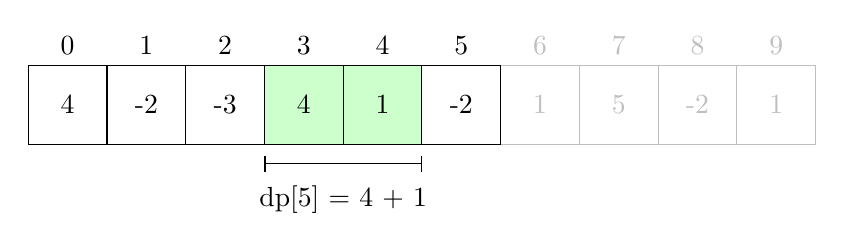
\begin{tikzpicture}
\foreach \x in {0,...,5}
  \node at (\x + 0.5, 1.25) {\x};
\foreach \x in {6,...,9}
  \node[gray!50!white] at (\x + 0.5, 1.25) {\x};
  
  
\fill[green!20!white] (3, 0) rectangle (5, 1);
\draw[gray!50!white] (6, 0) grid (10, 1);
\draw[] (0, 0) grid (6, 1);


\node at (0.5, 0.5) {4};
\node at (1.5, 0.5) {-2};
\node at (2.5, 0.5) {-3};
\node at (3.5, 0.5) {4};
\node at (4.5, 0.5) {1};
\node at (5.5, 0.5) {-2};
\node[gray!50!white] at (6.5, 0.5) {1};
\node[gray!50!white] at (7.5, 0.5) {5};
\node[gray!50!white] at (8.5, 0.5) {-2};
\node[gray!50!white] at (9.5, 0.5) {1};

\draw[|-|] (3, -0.25) -- (5, -0.25);
\node at (4, -0.7) {dp[5] = 4 + 1};
\end{tikzpicture}


\end{document}

